\documentclass[UTF8]{article}
\usepackage[margin=1in]{geometry} % 设置边距,符合Word设定
\usepackage{lipsum}
\usepackage{float}
\usepackage{amsmath}
\usepackage{tabularx}
\usepackage{graphicx}
\usepackage{amsfonts} 


\title{Appendix B. Parameters}
\author{LZU-CHINA}
\date{\today}
\begin{document}
    \maketitle
    \begin{abstract}
       This appendix show the parameters we applied to the model we establish. The parameters are determined by model assumptions, references, and estimation calculation.
       
%       We tested Raw Fluorescence Intensity and OD600 (Optical Density at 600 nm) in three scenarios of oleic acid concentrations: 5\%, 10\%, and 15\%, under both aerobic and anaerobic conditions. For each type, we conducted six sets of data. Subsequently, we organized and preprocessed the respective experimental data to aid in subsequent parameter estimation.
    \end{abstract}

\section{Model Review}

\subsection{Oleic acid induction system}

\begin{equation}
	\begin{aligned}
		\frac{d R}{d t} & =r_{\mathrm{x}, \mathrm{R}}-r_{\mathrm{seq}}-\lambda\left(E_{\mathrm{g}}\right) R, \\
		\frac{d D}{d t} & =r_{\mathrm{x}, \mathrm{D}}-\lambda\left(E_{\mathrm{g}}\right) D, \\
		\frac{d A}{d t} & =r_{\mathrm{D}}-r_{\mathrm{B}}-2 \cdot r_{\mathrm{seq}}-\lambda\left(E_{\mathrm{g}}\right) A, \\
		\frac{d C}{d t} & =r_{\mathrm{seq}}-\lambda\left(E_{\mathrm{g}}\right) C, \\
		\frac{d E_{\mathrm{g}}}{d t} & =r_{\mathrm{x}, E_{\mathrm{g}}}-\lambda\left(E_{\mathrm{g}}\right) \cdot E_{\mathrm{g}}, \\
		\frac{d F}{d t} & =r_{\mathrm{f}}.  \\
	\end{aligned}
\end{equation}

\subsection{Comparison of oleic acid inducer with native circuit}

\begin{equation}
	\text{Native circuit}: P_{\mathrm{R}}(R)= 
	\frac{a_{\mathrm{R}}}{1+K_{\mathrm{R}} R}\\
\end{equation}

\begin{equation}
	\text{Oleic acid inducer}: P_{\mathrm{R}}(R)=\left\{\begin{array}{cl}
		\frac{a_{\mathrm{R}}}{1+K_{\mathrm{R}} R}, & \text {for } R> \frac{1}{K_p} = 0.0033 \mu \mathrm{M} \cdot \mathrm{h}^{-1} \\
		\frac{a_{\mathrm{R}} K_{\mathrm{R}} R}{1+K_{\mathrm{R}} R}, & \text { for } R \leq \frac{1}{K_p} =  0.0033 \mu \mathrm{M} \cdot \mathrm{h}^{-1}
	\end{array}\right.
\end{equation}

\subsection{Parameter estimation}

\begin{equation}
	\begin{gathered}
		A F I=\frac{R F I}{O D 600} \\
		\text { Corrected } A F I_{n \%}=A F I_{n \%}-E m p t y
	\end{gathered}
\end{equation}

\begin{equation}
	\text{Exp} \ F_{n\%}  = A \cdot AFI_{n\%} + B
\end{equation}


\section{Parameters}


$$
\footnotesize
\begin{array}{|c|c|c|c|c|}
	\hline \text { Parameter description } & \text { Term } & \text { Value } & \text { Units } & \text { Reference } \\
	\hline \text { Forward sequestration } & k_{\mathrm{f}} & 612.55 & \mu \mathrm{M}^{-2} \cdot \mathrm{h}^{-1} & {[2]} \\
	\hline \text { Reverse sequestration } & k_{\mathrm{r}} & 900.73 & \mathrm{~h}^{-1} & {[2]} \\
	
	\hline \text { PlsB turnover rate } & k_{\text {cat }, \mathrm{B}} & 192.91 & h^{-1} & \text { [2] } \\
	\hline \text { FadD turnover rate } & k_{\text {cat }, \mathrm{D}} & 49 & h^{-1} & \text { [2] } \\
	\hline \text { FadR’strength to promote itself(NAR) } & a_{\mathrm{R}} & 0.0131 & \mu \mathrm{M} \cdot \mathrm{h}^{-1} & \text { [2] } \\
	\hline \text { FadR leaky expression (NAR) } & b_{\mathrm{R}} & 0.0007 & \mu \mathrm{M} \cdot \mathrm{h}^{-1} & {[2]} \\
	\hline \text { FadD’strength to promote itself } & a_{\mathrm{D}} & 0.0517 & \mu \mathrm{M} \cdot \mathrm{h}^{-1} & {[2]} \\
	
	\hline \text { FadD leaky expression } & b_{\mathrm{D}} & 0.0108 & \mu \mathrm{M} \cdot \mathrm{h}^{-1} & \text { [2] } \\
	
	\hline \begin{array}{l}
		\text { FadR affinity to own promoter } \\
		\text { (NAR) }
	\end{array} & K_{\mathrm{R}} & 4.3222 & \mu \mathrm{M}^{-1} & {[2]} \\
	
	\hline \text { FadR affinity to fadD} & K_{\mathrm{D}} & 305.95 & \mu \mathrm{M}^{-1} & \text { [2] } \\
	\hline \text { Michaelis constant } & K_{\mathrm{m}, \mathrm{B}} & 45429 & \mu \mathrm{M} & \text { [2] } \\
	\hline \text { Michaelis constant } & K_{\mathrm{m}, \mathrm{D}} & 0.0672 & \mu \mathrm{M} & \text { [2] } \\
	\hline \text { PlsB concentration } & B & 0.1369 & \mu \mathrm{M} & {[2]} \\
	\hline \text { Cell growth parameter } & \lambda_{\max } & 0.1818 & \mathrm{~h}^{-1} & {[2], \text { E. coli } \mathrm{DH} 1 \Delta \text { fadE strain. }} \\
	\hline E_{\mathrm{g}} \text { promoter strength } & a_{\mathrm{g}} & \lambda_{\max } & \mu \mathrm{M} \cdot \mathrm{h}^{-1} & \text { To ensure full express at } \lambda_{\max } \text {. } \\
	\hline \text { FadR’strength to promote itself(PAR) } & a_{\mathrm{R}} & 0.0131 & \mu \mathrm{M} \cdot \mathrm{h}^{-1} & \text { Same as NAR by assumption} \\
	\hline \text { FadR leaky expression (PAR) } & b_{\mathrm{R}} & 0.0007 & \mu \mathrm{M} \cdot \mathrm{h}^{-1} & \text { Same as NAR by assumption  } \\
	\hline \text { Decrease paramameter in growth } & s_{\mathrm{T}} & 0.7 & - & \text { [3], By pgi down-regulation.} \\
	\hline \begin{array}{l}
		\text { FadR affinity to own promoter } \\
		\text { (PAR) }
	\end{array} & K_{\mathrm{R}} & \begin{array}{l}
		4.3222 \times 7
	\end{array} & \mu \mathrm{M}^{-1} & \begin{array}{l}
		\text {Multiple times the value of NAR }
	\end{array} \\
	\hline \text { FadR affinity to } E_{\mathrm{g}} \text { promoter } & K_{\mathrm{g}} & \begin{array}{l}
		=K_{\mathrm{R}}= \\
		4.9114
	\end{array} & \mu \mathrm{M}^{-1} & \begin{array}{l}
		\text { the same promoter as FadR with PAR} 
	\end{array} \\
	\hline \begin{array}{l}
		\text { Affinity of FadR for prod synthesis } \\
		\text { enzyme } E_{\mathrm{p}}
	\end{array} & K_{\mathrm{p}} & \begin{array}{l}
		=K_{\mathrm{D}}= \\
		305.95
	\end{array} & \mu \mathrm{M} \cdot \mathrm{h}^{-1} & \begin{array}{l}
		\text { [1], Designed with FadR operator} \\
		\text { site from fadD promoter. }
	\end{array} \\
	\hline
	\text{Aerobic coefficient } & A_{\text{ae}} & 1.59 & - & \text{Parameter estimation calculation} \\
	\hline
	\text{Aerobic intercept } & B_{\text{ae}} & 1.82 & - & \text{Parameter estimation calculation} \\
	\hline
	\text{Anaerobic coefficient } & A_{\text{an}} & 1.73 & - & \text{Parameter estimation calculation} \\
	\hline
	\text{Anaerobic intercept} & B_{\text{an}} & 0.98 & - & \text{Parameter estimation calculation} \\
	\hline
\end{array}
$$

\begin{figure}[h]
	\centering
	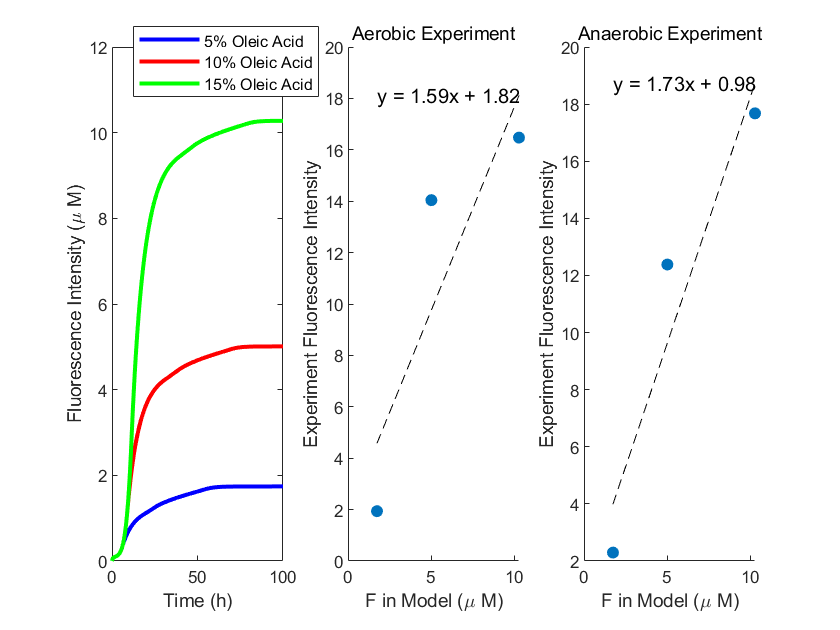
\includegraphics[width=0.75\linewidth]{figures/para_fit_fig.png}
	\caption{Parameter estimation by measuring the fluorescence intensity and fitting}
	\label{fig:parafit}
\end{figure}

%$
%A_aero = 1.59, B_aero = 1.82, A_anaero = 1.73, B_anaero = 0.98
%$

\end{document}